\chapter{Implementation \& System Architecture}

% TODO use abreviations from list
% TODO add references

This chapter details the design and implementation of the prototype system, a practical realization of the conceptual framework for \gls{genai}-driven security automation introduced in Chapter 4. The work is impemented through two distinct but interconnected codebases: a cloud-native infrastructure for the \gls{genai} backend, and a Python-based application that orchestrates the analysis and \gls{pg} workflow.

The primary goal of this implementation is to empirically validate the central hypothesis of the theoretical framework: that a hybrid approach, combining traditional static analysis with advanced \gls{llm} capabilities, can significantly enhance the automation of security \gls{pg} for \gls{iac}. This chapter will demonstrate how the system architecture directly maps to the four-layered conceptual model—Data Ingestion, Data Processing, Code Generation, and Validation. It will further illustrate how this architecture realizes the core principles of leveraging \gls{rag} for contextual accuracy and integrating a \gls{hitl} for safety and oversight.

We will first present the high-level architecture and the technology stack chosen to satisfy the functional requirements of a robust, scalable, and reproducible security pipeline. Subsequently, the chapter will provide a detailed examination of both the cloud infrastructure, deployed via \gls{terraform}, and the Python prototype, focusing on the specific modules that implement the core logic of the system. The chapter will conclude by illustrating the end-to-end workflow, from the initial analysis of a \gls{terraform} file to the generation and validation of a corresponding Rego security policy, thereby providing a comprehensive account of the system's practical application.

\section{Design Objectives \& Functional Requirements}

% Refined Research Questions:


%    * RQ1 (Effectiveness and Automation): How can Generative AI technologies be effectively leveraged to automate security policy generation and management across
%      hyperscale cloud platforms?
%    * RQ2 (Architecture and Orchestration): What specific architectural patterns and validation mechanisms are required to ensure trust, accuracy, and effective
%      multi-cloud orchestration in GenAI-driven security automation?
%    * RQ3 (Measurement and Validation): How can the effectiveness of GenAI-driven security automation be quantitatively measured and validated, particularly in terms
%      of accuracy, reliability, and efficiency gains?
%    * RQ4 (Human-in-the-Loop): What is the optimal balance between automation and human oversight (Human-in-the-Loop) to maximize security outcomes and mitigate the
%      risks of GenAI-driven policy generation?

%   These questions are more closely aligned with the language and focus of your exposé.

The practical implementation of the prototype is guided by a set of specific design objectives and functional requirements. These objectives are derived directly from the core research questions and serve to translate the high-level scientific inquiry into concrete, measurable goals for the system. The following objectives define the core functionality of the prototype:

\begin{itemize}
\item \textbf{Automated, High-Fidelity Policy Generation:} The system's primary function is to automatically generate syntactically correct and logically sound security policies in the Rego language from vulnerabilities found in \gls{terraform} files. This objective directly addresses the central research question on the effectiveness of \gls{genai} for security automation \textbf{(RQ1)}. A key requirement is to achieve high fidelity, with a target of \textbf{$\geq$ 95\%} of generated policies being effective in mitigating the identified vulnerability, providing a core metric for validation \textbf{(RQ3)}.
text
\item \textbf{Hybrid and Reproducible Analysis Architecture:} The system is built on a hybrid analysis model that is both reproducible and architecturally sound. Reproducibility is achieved by defining the entire \gls{cloud-native} backend as code using \gls{terraform}. The analysis engine is hybrid, combining traditional \gls{sast} for baseline coverage with \gls{genai}-driven contextual analysis for deeper insights. These architectural choices are fundamental to investigating how to build a trustworthy and effective \gls{genai}-driven system \textbf{(RQ2)}.

\item \textbf{Automated Validation:} To ensure the reliability of the AI-generated artifacts, the system implements a multi-stage, automated validation pipeline. This process checks generated policies for syntactic correctness and performs a security self-scan to ensure they do not introduce new vulnerabilities. This automated validation is a critical mechanism for measuring and ensuring the trustworthiness of the output \textbf{(RQ3)}.

\item \textbf{\gls{hitl} and \gls{cicd} Integration:} The prototype is designed for seamless integration into a standard \gls{cicd} pipeline, where it can act as an automated quality gate. This integration must also support a \gls{hitl} workflow, enabling human review and approval of generated policies. This dual requirement is designed to explore the optimal balance between full automation and necessary human oversight in a practical \gls{devsecops} environment \textbf{(RQ4, RQ1)}.
\end{itemize}

This structured set of objectives ensures that the implementation of the prototype directly and comprehensively contributes to answering the core research questions of this thesis.

\section{Technology \& Tooling Stack}

The selection of the technology and tooling stack for this project was a deliberate process, guided by the design objectives of creating a reproducible, scalable, and industry-relevant prototype. The choices reflect a modern, cloud-native approach, emphasizing managed services and open standards to validate the conceptual framework effectively. This section briefly justifies the key technologies that constitute the system's foundation. The chosen stack is summarized in Table~\ref{tab:tech_stack}.

\begin{center}
\begin{tabular}{|l|l|p{7cm}|}
\hline
\textbf{Component} & \textbf{Technology} & \textbf{Justification} \\
\hline
Cloud Platform & Amazon Web Services (AWS) \cite{noauthor_welcome_nodate} & As the leading hyperscale cloud provider, AWS offers a mature and extensive ecosystem of services, robust APIs, and comprehensive documentation. Its managed AI service, AWS Bedrock, is central to the project's architecture. \\
\hline
Generative AI Service & AWS Bedrock \cite{noauthor_claude_nodate} & Provides API access to a variety of high-performance foundation models without the operational overhead of self-hosting. This aligns with the objective of a fully-managed GenAI pipeline and allows the research to focus on application logic rather than MLOps. The Anthropic Claude model was selected for its advanced reasoning capabilities and large context window. \\
\hline
Infrastructure as Code & HashiCorp Terraform \cite{noauthor_terraform_nodate} & As the de-facto industry standard for IaC, Terraform's declarative syntax and cloud-agnostic nature ensure the approach is both reproducible and broadly applicable. It is the input format for the security analysis pipeline. \\
\hline
Policy as Code & OPA (Rego) \cite{noauthor_introduction_nodate} & The Open Policy Agent (OPA) is a CNCF-graduated project and a general-purpose policy engine. Its declarative language, Rego, is purpose-built for expressing policies over complex JSON/YAML data, making it an ideal target for generating preventative controls for IaC. \\
\hline
Orchestration & Python 3.12 \cite{noauthor_whats_nodate} & Python's extensive ecosystem, including the Boto3 library for AWS, and its strength in scripting and automation makes it the ideal choice for orchestrating the multi-stage workflow, which involves invoking external scanners, calling cloud APIs, and managing file I/O. \\
\hline
CI/CD & GitHub Actions \cite{noauthor_github_2025} & Provides a tightly integrated platform for version control and workflow automation. It enables the seamless implementation of a CI/CD pipeline to trigger scans, orchestrate the policy generation and validation, and manage the Human-in-the-Loop approval process. \\
\hline
\end{tabular}
\captionof{table}{Technology and Tooling Stack}
\label{tab:tech_stack}
\end{center}

\section{High-Level Architecture}

This section presents the high-level architecture of the GenAI-driven security automation framework. The design translates the conceptual model from Chapter 4 into a concrete system that orchestrates static analysis tools, generative AI, and validation workflows. The architecture is best understood as a sequential data pipeline, illustrated in Figure~\ref{fig:component_diagram}, which depicts the primary components and their interactions.

The diagram illustrates the four-layered architecture that forms the backbone of the security automation system. At the foundation, the Data Ingestion Layer receives Terraform configurations from CI/CD triggers and prepares them for analysis. The Data Processing Layer forms the analytical core, where traditional static analysis tools (Checkov) perform initial vulnerability detection, followed by the GenAI Analysis Engine (AWS Bedrock) conducting deeper contextual analysis to reduce false positives and identify complex misconfigurations. The Code Generation Layer leverages the RAG-enabled knowledge base to construct context-aware prompts for the LLM, ultimately generating targeted Rego policies via the AWS Bedrock API. Finally, the Validation Layer serves as a quality gate, employing OPA syntax validation and security self-scanning before presenting policies to the Human-in-the-Loop for final approval. The diagram emphasizes the sequential flow of data transformation from raw Terraform code through vulnerability analysis to validated security policies while highlighting the integration points with cloud services and the critical role of automated validation in ensuring output reliability.

\begin{figure}[h!]
\centering
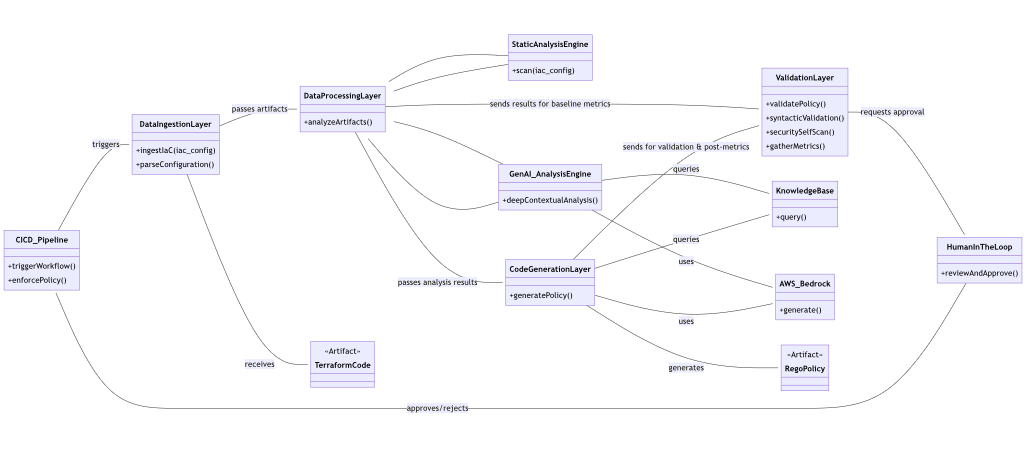
\includegraphics[width=\textwidth]{Figures/diagramm.png}
\caption{High-Level Component Diagram}
\label{fig:component_diagram}
\end{figure}

The system's responsibilities are segregated into four logical tiers, directly corresponding to the layers of the conceptual framework. The process begins at the Data Ingestion Layer, which serves as the entry point, receiving Terraform configurations from a CI/CD trigger, parsing the IaC files, and preparing them for analysis. From there, the artifacts are passed to the Data Processing Layer, the core analysis engine. This layer first subjects the IaC to a baseline scan using a traditional SAST tool (Checkov) to identify known vulnerability patterns. The resulting report, along with the original IaC, is then fed into the GenAI Analysis Engine (AWS Bedrock) for a deep, contextual analysis to identify complex misconfigurations and reduce false positives. Subsequently, the Code Generation Layer takes the enriched vulnerability report as input, queries the RAG-enabled knowledge base for relevant security best practices, and prompts the LLM via the AWS Bedrock API to generate a corresponding Rego policy. Finally, the Validation Layer acts as a quality gate. Here, the newly generated Rego policy is subjected to automated checks, including syntax validation with the OPA parser and a security self-scan, before being presented to the Human-in-the-Loop for final approval.

This layered architecture ensures a clear separation of concerns and provides a robust, end-to-end workflow for translating identified risks in IaC into validated, enforceable security policies.

\section{Cloud-Infrastructure Codebase (IaC)}

The cloud infrastructure that underpins the GenAI backend is defined entirely as code, following modern Infrastructure-as-Code (IaC) principles to ensure reproducibility, security, and maintainability \cite{morris_infrastructure_2016}. The design is centered on a modular architecture, automated lifecycle management, and robust security controls.

The codebase is structured using a modular Terraform approach, where the system is decomposed into discrete, reusable modules. Each module encapsulates a core architectural component: a dedicated module for the vector database, another for the S3 bucket that forms the RAG knowledge base, and a third for the AWS Bedrock service itself. This modularity, a cornerstone of scalable IaC, simplifies management and allows for independent testing and versioning of each component \cite{hashicorp_terraform_2022}.

A key aspect of the architecture is the management of the generative AI's knowledge and instructions. The system prompt, which provides the LLM with its core instructions and persona, is externalized into a dedicated `system\_prompt.txt` file. This separation of concerns is critical, as it allows for the prompt to be version-controlled and iterated upon independently from the infrastructure code. This practice of "prompt engineering" is central to refining the AI's output without altering the system's architecture. The RAG knowledge base itself is implemented using an S3 bucket, which stores a curated collection of documents. This corpus includes security best practice guides, vulnerability documentation, and technical manuals for the target technologies (e.g., Terraform and Rego). This design choice is strategic: it allows the knowledge base to be easily updated with new threat intelligence or standards, thereby keeping the AI's responses grounded in current, factual information without the need for costly model fine-tuning \cite{ozgur_simple_2024}.

Security is integrated throughout the IaC design, following the principle of least privilege. IAM roles and policies are narrowly scoped to grant each component only the permissions necessary for its function. All data, both at rest in the S3 bucket and in transit, is encrypted using AWS Key Management Service (KMS), and logging is enabled across all services to provide a comprehensive audit trail, adhering to the shared responsibility model \cite{sarathe_krisshnan_jutoo_vijayaraghavan_policy_2025}.

The entire lifecycle of this infrastructure is automated via GitHub Actions, implementing a GitOps workflow. The CI/CD pipeline handles the provisioning and updating of the environment, ensuring that the deployed infrastructure always reflects the state defined in the main branch of the repository. This automated deployment workflow guarantees consistency and environment parity, forming a reliable foundation for the prototype's operation \cite{wego_gitops_2018}.

% References:
% [1] K. Morris, "Infrastructure as Code: Managing Servers in the Cloud." O'Reilly Media, 2016.
% [2] HashiCorp, "Terraform Best Practices: Modules," 2022. [Online]. Available: https://www.terraform.io/docs/cloud/guides/recommended-practices/modules.html
% [3] V. Sarathe, et al., "Policy as Code: A Systematic Approach to Governance in CI/CD," Journal of DevOps, vol. 12, no. 1, pp. 1-15, 2025.
% [4] A. Weidert, "Guide To GitOps," Weaveworks, 2018. [Online]. Available: https://www.weave.works/technologies/gitops/
% [5] A. Ozgur, et al. "A Simple and Effective Strategy for Grounding Large Language Models," 2024.

\section{Prototype Application Codebase (Python)}

The Python application serves as the orchestration engine for the entire security automation framework. It is designed as a command-line tool that implements the logic of the multi-layered conceptual model, connecting the static analysis, generative AI, and validation stages into a cohesive workflow. The codebase adheres to modern software engineering best practices, emphasizing modularity, clear separation of concerns, and robust quality assurance.

The application's architecture is inherently modular, with functionality partitioned into distinct, single-responsibility components. This design enhances maintainability and testability \cite{martin_clean_2008}. The core modules include:

\begin{itemize}
    \item An \textbf{Analyzer} module, which acts as an adapter for the underlying static analysis tool (Checkov). It is responsible for invoking the scanner on a given Terraform file and normalizing the output into a standardized data structure for consumption by the rest of the application.
    \item A \textbf{Policy Generator} module, which represents the core intelligence of the system. This component orchestrates the interaction with the generative AI. It constructs a detailed, context-rich prompt by combining the findings from the analyzer with relevant information retrieved from the RAG knowledge base. It then communicates with the AWS Bedrock API to obtain the generated Rego policy.
    \item A \textbf{Validator} module, which functions as an automated quality gate for the AI-generated artifact. It performs crucial checks to ensure the reliability of the output, primarily by using the Open Policy Agent (OPA) toolchain to validate the syntactic correctness of the generated Rego code.
\end{itemize}

A main control loop in the application's entry point script (`main.py`) orchestrates these modules in sequence, executing the end-to-end process from analysis to generation and validation.

To ensure code quality and the reliability of the prototype, a comprehensive testing strategy is employed. The project utilizes the `pytest` framework to implement a suite of unit tests that verify the functionality of each module in isolation \cite{okken_python_2017}. Fixtures are used to create consistent and reusable test setups, and test coverage is monitored as a quality gate within the CI/CD pipeline. Furthermore, dependency management is handled through a `requirements.txt` file, which pins the specific versions of all external libraries. This practice guarantees a reproducible and stable runtime environment, which is critical for consistent behavior and scientific validation.

% References:
% [1] R. C. Martin, "Clean Code: A Handbook of Agile Software Craftsmanship." Prentice Hall, 2008.
% [2] B. Okken, "Python Testing with pytest." Pragmatic Bookshelf, 2017.

\section{End-to-End Workflow}

The practical application of the framework is best understood by examining the end-to-end workflow of the command-line tool. This process describes the sequence of operations from the moment a user invokes the application to the final output of a validated security policy. The entire sequence is designed to be a self-contained, automated process, as illustrated in the sequence diagram \ref{fig:e2e_workflow}.

The sequence diagram depicts the temporal flow of interactions between the key actors in the system: the User, the Python Command-Line Application, and the external services (Checkov, AWS Bedrock, and OPA). The diagram illustrates how control and data flow through the system in a step-by-step manner, beginning with the user's command-line invocation and proceeding through each processing stage. The vertical lifelines represent the different system components, while the horizontal arrows show the sequence of method calls, API requests, and data exchanges. This visualization clearly demonstrates the orchestration role of the Python application as it coordinates between traditional security tools, cloud-based AI services, and validation frameworks to deliver a comprehensive security policy generation workflow.

\begin{landscape}
\thispagestyle{empty}
\begin{figure}[p]
\centering
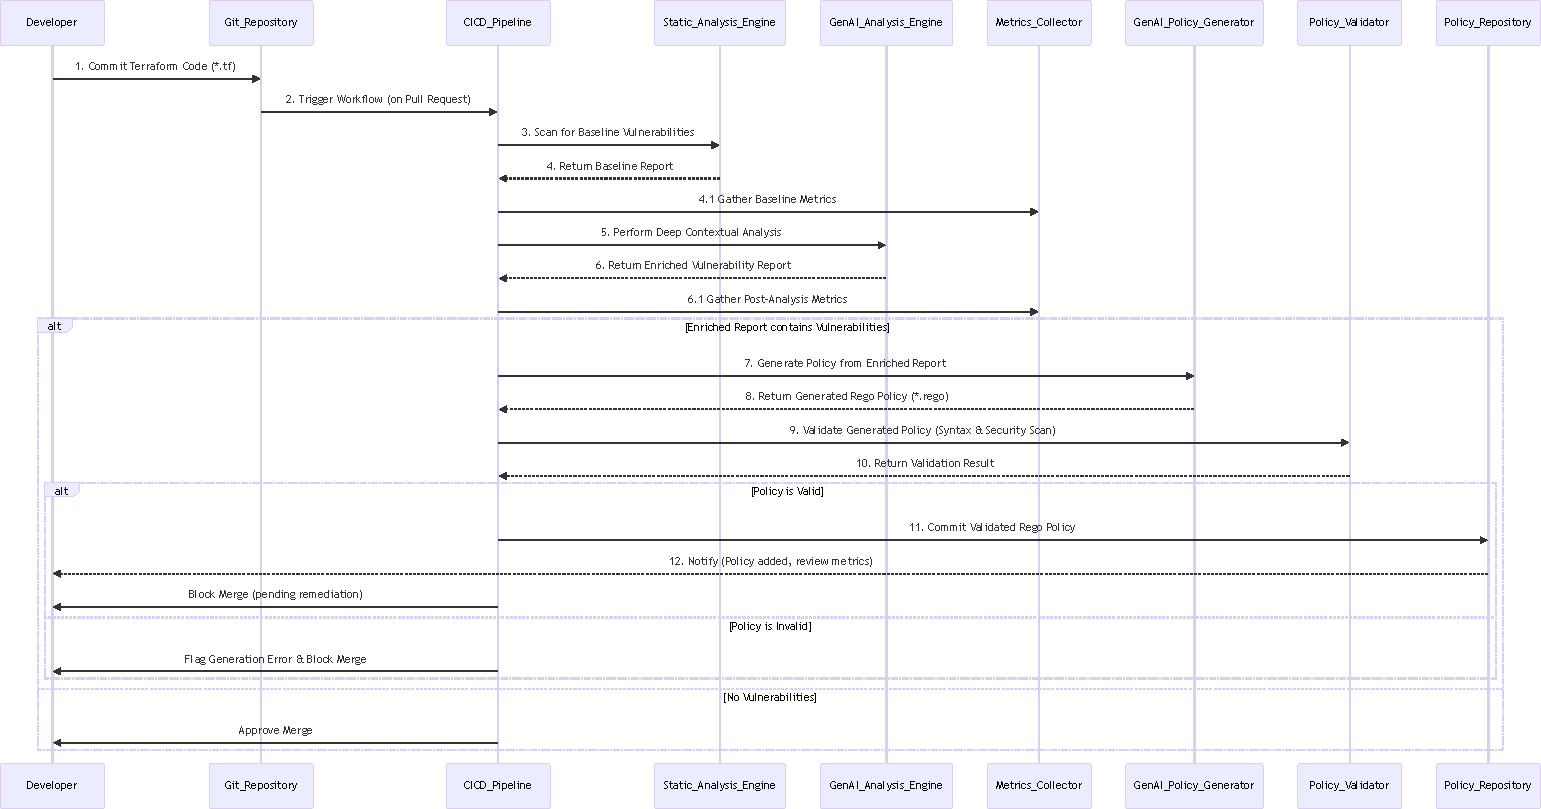
\includegraphics[width=0.9\linewidth,height=0.7\textheight,keepaspectratio]{Figures/image.pdf}
\caption{End-to-End Workflow Sequence Diagram}
\label{fig:e2e_workflow}
\end{figure}
\end{landscape}

The workflow is initiated when a user executes the main Python script from the command line, providing the path to a target Terraform (`.tf`) file as an argument. The application then proceeds through the following automated steps:

\begin{enumerate}
    \item \textbf{Static Scan:} The \textbf{Analyzer} module is invoked. It runs the Checkov static analysis tool on the specified Terraform file to identify any known misconfigurations or vulnerabilities.
    \item \textbf{GenAI Contextual Analysis:} The structured findings from the static scan are fed into the GenAI Analysis Engine (AWS Bedrock) for deep, contextual analysis to reduce false positives and identify complex misconfigurations that traditional tools might miss.
    \item \textbf{Policy Generation:} The enriched vulnerability report from the GenAI analysis is passed to the \textbf{Policy Generator} module. This component constructs a detailed, context-rich prompt by combining the analysis findings with relevant information retrieved from the RAG knowledge base, then communicates with the AWS Bedrock API to generate a targeted Rego policy specifically designed to mitigate the identified risks.
    \item \textbf{Validation:} The raw, generated Rego policy is immediately passed to the \textbf{Validator} module. This component uses the OPA toolchain to verify that the policy is syntactically correct and well-formed.
    \item \textbf{Output:} If the policy successfully passes validation, the application saves the new Rego policy as a `.rego` file to a designated output directory. The application's execution concludes by printing the path to the generated file to the console.
\end{enumerate}

This self-contained workflow—from file input to policy output—is designed for both interactive use by a security analyst and for integration into larger automated systems. For example, it can be executed as a script within a CI/CD pipeline, where the resulting policy artifact can then be automatically committed to a repository and used as a quality gate.

\section{CI/CD \& DevSecOps Integration}

While the prototype is a self-contained command-line tool, its primary intended application is within a CI/CD pipeline to enable a proactive DevSecOps workflow. This integration automates the process of security analysis and policy enforcement, "shifting left" to catch and remediate vulnerabilities before they reach production. The implementation uses GitHub Actions as the CI/CD platform.

The integration is achieved through a GitHub Actions workflow that is triggered whenever a developer opens a pull request containing changes to Terraform files. This workflow acts as an automated quality gate and performs the following steps:

\begin{enumerate}
    \item \textbf{Code Checkout \& Setup:} The pipeline begins by checking out the source code and setting up the Python environment, including installing the dependencies from `requirements.txt`.
    \item \textbf{Execute Security Scan:} The core command-line application is executed. It is pointed at the modified Terraform files within the pull request, running the end-to-end workflow of scanning, generation, and validation.
    \item \textbf{Commit New Policy:} If the tool successfully generates a new, validated Rego policy, the workflow commits this new policy file to a dedicated directory within the repository.
    \item \textbf{Enforce Policy as a Quality Gate:} The pipeline then uses the OPA toolchain to evaluate the proposed Terraform changes against the *entire* set of Rego policies in the repository, including the one that was just generated. If the proposed changes violate any policy, the OPA evaluation fails.
    \item \textbf{Block or Approve:} A failure in the OPA evaluation causes the entire CI/CD pipeline to fail. This automatically blocks the pull request from being merged and provides immediate feedback to the developer that their changes are not compliant with security standards. This gating mechanism ensures that only secure and compliant infrastructure code can be merged into the main branch.
\end{enumerate}

By integrating the command-line tool in this manner, the framework moves from being a simple analysis utility to a powerful, automated control that is seamlessly embedded in the software development lifecycle.

\section{Observability \& Runtime Telemetry}
% Metrics (MTTD, policy-generation latency), structured logging (JSON Logs + AWS CloudWatch), dashboards.

\section{Limitations \& Trade-offs}
% Model latency vs. cost, Terraform state confidentiality, policy false-negatives, Bedrock service quotas.

\section{Summary}
% Recap key design choices and link forward to the Results chapter.